\documentclass[../characterization.tex]{subfiles}
\graphicspath{{\subfix{../../../../images/}}}
\begin{document}
    \textbf{Fourier Transform Infrared Spectroscopy (FTIR)} is a widely used analytical technique that provides 
    information about the chemical bonds and molecular structure of materials, including nanophosphors. It is 
    based on the principle of measuring the absorption, transmission, or reflection of infrared (IR) light by the 
    sample over a range of frequencies.FTIR is a versatile and non-destructive technique used to characterize 
    nanophosphors and understand their chemical composition, molecular structure, and functional groups. It is 
    widely employed in materials science, chemistry, pharmaceuticals, and many other fields for quality control, 
    material identification, and chemical analysis.
    \begin{Figure}
        \centering
        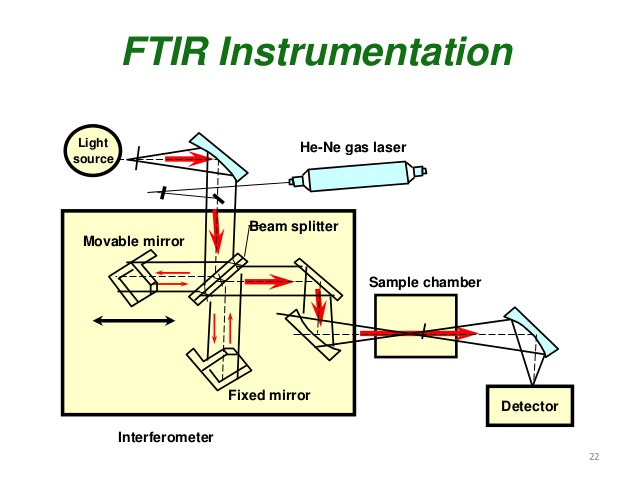
\includegraphics[width=0.4\linewidth]{ftir.jpg}
        \captionof{figure}{Fourier Transform Infrared Spectroscopy (FTIR) instrumentation\cite{u14}}\label{fig:ftir}
    \end{Figure}
    FTIR utilizes infrared radiation, which falls in the region of the electromagnetic spectrum between visible 
    light and microwaves. This region corresponds to the vibrational and rotational energy levels of molecules, 
    allowing for the analysis of chemical bonds and functional groups. For FTIR analysis, nanophosphor samples are 
    typically ground into a fine powder and mixed with an IR-transparent matrix, such as potassium bromide (KBr), 
    to form a solid pellet. The pellet is then placed in the IR spectrometer for analysis. When IR light interacts 
    with the sample, it is absorbed by the molecular bonds, causing the atoms within the bonds to vibrate. 
    Different chemical bonds and functional groups exhibit characteristic vibrational frequencies, which 
    correspond to specific IR wavelengths.In FTIR, the IR light passing through the sample is split into two 
    beams. One beam passes through the sample, and the other passes through a reference mirror. The two beams are 
    then recombined, and their interference pattern is measured. This technique allows for the acquisition of the 
    entire IR spectrum simultaneously.The interference pattern is transformed using a mathematical technique 
    called Fourier transform, resulting in the acquisition of the sample's IR spectrum. The spectrum represents 
    the absorption or transmission of IR light at different wavelengths/frequencies, providing information about 
    the molecular vibrations and chemical groups present in the nanophosphor.


\end{document}